% !TeX spellcheck = it_IT
\documentclass[italian,11pt,a4paper,twoside,openright]{book}
\usepackage[lmargin=142pt,rmargin=95pt,tmargin=127pt,bmargin=123pt]{geometry}
\usepackage[utf8]{inputenc}
\usepackage{graphicx}
\usepackage{siunitx}
\usepackage{babel}
\usepackage{mathtools}
\usepackage{amsmath}
\usepackage{amssymb}
\usepackage{pgf,tikz}
\usepackage{hyperref}
\usepackage{minted}
\usepackage{tabu}
\usepackage{cleveref}
\usepackage{float}
\usepackage{cite}
\usepackage{enumitem}
\usepackage{microtype}
\usepackage{setspace} % for \setstretch
\usepackage[T1]{fontenc}
\usepackage{lmodern} % \scshape
\usepackage{titling} % \thetitle


\setlist[itemize]{noitemsep, topsep=5pt, leftmargin=*}
	
\usetikzlibrary{matrix, positioning, arrows.meta}
\newlength{\myheight}
\setlength{\myheight}{2.5cm}
\tikzset{labels/.style={font=\sffamily\scriptsize},
	circuit/.style={draw,minimum width=2cm,minimum height=\myheight,very thick,inner sep=1mm,outer sep=0pt,cap=round,font=\sffamily\bfseries},
	triangle 45/.tip={Triangle[angle=45:8pt]}
}


\newcommand{\code}[1]{\texttt{#1}} 

% Some definitions.
\def\advisor#1{\gdef\@advisor{#1}}
\def\mastername#1{\gdef\@mastername{#1}}
\def\coadvisorOne#1{\gdef\@coadvisorOne{#1}}
\def\coadvisorOneUniversity#1{\gdef\@coadvisorOneUniversity{#1}}
\def\coadvisorTwo#1{\gdef\@coadvisorTwo{#1}}
\def\committeeInternal#1{\gdef\@committeeInternal{#1}}
\def\committeeInternalOne#1{\gdef\@committeeInternalOne{#1}}
\def\committeeInternalTwo#1{\gdef\@committeeInternalTwo{#1}}
\def\committeeExternal#1{\gdef\@committeeExternal{#1}}
\def\degreeyear#1{\gdef\@degreeyear{#1}}
\def\degreemonth#1{\gdef\@degreemonth{#1}}
\def\degreeterm#1{\gdef\@degreeterm{#1}}
\def\degree#1{\gdef\@degree{#1}}
\def\department#1{\gdef\@department{#1}}
\def\field#1{\gdef\@field{#1}}
\def\university#1{\gdef\@university{#1}}
\def\universitycity#1{\gdef\@universitycity{#1}}
\def\universitystate#1{\gdef\@universitystate{#1}}
\def\programname#1{\gdef\@programname{#1}}
\def\pdOneName#1{\gdef\@pdOneName{#1}}
\def\pdOneSchool#1{\gdef\@pdOneSchool{#1}}
\def\pdOneYear#1{\gdef\@pdOneYear{#1}}
\def\pdTwoName#1{\gdef\@pdTwoName{#1}}
\def\pdTwoSchool#1{\gdef\@pdTwoSchool{#1}}
\def\pdTwoYear#1{\gdef\@pdTwoYear{#1}}
% School name and location
\university{University of Padova}
\universitycity{Padova}
\universitystate{Italy}

% School color found from university's graphic identity site:
% http://www.nyu.edu/employees/resources-and-services/media-and-communications/styleguide.html
\definecolor{SchoolColor}{rgb}{0.71, 0, 0.106} % UNIPD red
\definecolor{chaptergrey}{rgb}{0.61, 0, 0.09} % dialed back a little
\definecolor{midgrey}{rgb}{0.4, 0.4, 0.4}

\hypersetup{
	colorlinks,
	citecolor=SchoolColor,
	filecolor=black,
	linkcolor=black,
	urlcolor=SchoolColor,
	pdftitle={Implementazione di un sintetizzatore musicale su scheda Nexys4 DDR}
}


\renewcommand{\frontmatter}{
	\pagenumbering{roman}
	\maketitle
	\frontispiece
	\clearpage
}

\begin{document}

\author{Enrico Lumetti}
\title{Implementazione di un sintetizzatore musicale su scheda Nexys4 DDR}
%\title{Implementation of a musical synthesizer on the Nexys 4 DDR board}
%\title{Sintesi audio su scheda FPGA Nexys 4 DDR}
%\title{Audio Synthesis on the Nexys 4 DDr FPGA board}
%\title{Implementazione di un sintetizzatore MIDI digitale su scheda FPGA Nexys 4 DDR}
%\title{Implementation of a MIDI synthesizer on the Nexys 4 DDR FPGA board}
\advisor{Daniele Vogrig}
\mastername{Ingegneria dell'Informazione}
\date{15 Luglio 2019}


\thispagestyle{empty}
\begin{center}
	\vbox to0pt{\vbox to\textheight{\vfill 
\includegraphics[width=11.5cm]{resources/unipd-light} \vfill}\vss}
	%\vspace*{\fill}
	\begin{figure}
		\centering
		
\includegraphics[height=2.5cm]{resources/unipd-bn}
	\end{figure}
	
	\setstretch{1.5}
	
	\scshape{\Large{\bfseries{Università degli Studi di Padova}}} \\
	\line(1, 0){400} \\
	\scshape{\large{Dipartimento di ingegneria dell'informazione}} \\
	
	\vspace{5pt}
	\small{\textit{Tesi di laurea in}}
	\@mastername
	
	\setstretch{3}
	
	\vspace{40pt}
	\scshape{\LARGE{\bfseries{\textcolor{SchoolColor}{\thetitle}}}} \normalsize \\
	\vspace{25pt}
	\vspace{15pt}
	\scshape{Anno Accademico 2018/19} \\
	\scshape{15 Luglio 2019}
	\setstretch{1.2}
	
	\vfill
	\begin{normalsize}
		\begin{flushleft}
			\textit{Relatore} \hfill \textit{Candidato}\\
			\vspace{1pt}
			Daniele Vogrig \hfill Enrico Lumetti\\
			Università di Padova \\
			\vspace{6pt}
			
		\end{flushleft}
	\end{normalsize}
	
\end{center}
\vspace*{\fill}
\singlespacing
\pagenumbering{gobble} 
\cleardoublepage

\pagenumbering{roman}
\chapter*{Abstract}
Il successo dei sintetizzatori in ambito musicale dagli anni 70 in poi è
è stato determinante per l'industria musicale. Grazie alla loro versatilità
i sintetizzatori permettono di riprodurre svariati suoni, spesso
programmabili dal musicista, e ampliano enormemente le possibilità espressive.
Con l'avvento dell'elettronica digitale quasi tutti i sintetizzatori in
commercio hanno cominciato a fare uso di tecniche di sintesi digitale e
dei microprocessori.
In questa tesi ci si propone di realizzare un semplice sintetizzatore 
digitale polifonico e con sintesi a wavetable, comandabile attraverso
il protocollo MIDI.
Per la realizzazione del sintetizzatore si farà uso di una scheda
Nexys4 DDR, contenente una FPGA Xilinx Artix 7, un dispositivo programmabile
molto diverso da un convenzionale processore e programmato attraverso
il linguaggio di descrizione dell'hardware VHDL.

\tableofcontents
\mainmatter
\chapter{Introduzione}
Lo scopo di questa tesi è di descrivere la realizzazione di un sintetizzatore
musicale implementato su una scheda Nexys 4 DDR della Digilent.
La particolarità di quest'ultima è la presenza, al suo interno, di una FPGA,
un circuito programmabile molto diverso da un convenzionale microprocessore
o microcontrollore.
Una FPGA, infatti, si programma con linguaggi di descrizione dell'hardware (HDL)
che descrivono la struttura e il funzionamento di un circuito digitale.
Il sintetizzatore presenta le seguenti caratteristiche:
\begin{itemize}
   \item polifonia
   \item sintesi basata su wavetable (forma d'onda campionata)
   \item supporto del protocollo MIDI
   \item audio monofonico
\end{itemize}

Oltre all'architettura realizzata, vengono discusse in questo lavoro la teoria
dietro alla sintesi digitale del segnale sonoro e della PWM utilizzata
per pilotare l'uscita audio.
Infine si dà una caratterizzazione delle performance del sintetizzatore in termini
di signal-to-noise ratio.

\section{Descrizione di un sintetizzatore musicale}
Un sintetizzatore musicale permette la riproduzione di suoni di carattere, intensità e frequenza controllabili dal musicista.
L'utilizzo dei sintetizzatori come strumento, sia in studio che dal vivo, si afferma negli anni settanta grazie all'invenzione del \textit{Minimoog}, meno costoso e voluminoso dei sintetizzatori a muro degli anni sessanta.
Il \textit{Minimoog} era un sintetizzatore analogico e monofonico, cioè capace di riprodurre solamente una nota alla volta, al contrario dei moderni sintetizzatori detti \textit{polifonici}.
Al giorno d'oggi i sintetizzatori sono per la maggior parte implementati in maniera digitale e permettono l'utilizzo di una varietà di tecniche di sintesi del suono.
In questa tesi ci si occuperà di un semplice sintetizzatore polifonico, capace di riprodurre forme d'onda campionate e controllabile attraverso il protocollo MIDI (Musical Instrument Digital Interface), ampiamente diffuso nell'industria musicale.
La scheda Nexys 4 DDR utilizzata per il progetto è dotata di una porta seriale usata per comandare il sintetizzatore
 e di un uscita mini-jack a singolo canale.

\section{La catena del segnale del sintetizzatore}
L'input di un sintetizzatore viene dato dal musicista attraverso uno
strumento fisico. Lo strumento invia al sintetizzatore un segnale di
controllo che specifica quali note suonare, a che intensità, quali sono
i parametri dello strumento, ecc. A tale scopo è universalmente impiegato
lo standard MIDI, che specifica sia il protocollo di comunicazione che
le caratteristiche elettriche della connessione fisica.
Il sintetizzatore si occuperà di riprodurre i suoni desiderati. Due caratteristiche fondamentali del suono riprodotto sono la sua frequenza e il suo timbro. Per variare queste due componenti sono disponibili una varietà di tecniche.
In questo progetto ci si avvale della \textit{Direct Digital Frequency Synthesis} per la generazione di una frequenza determinata, mentre si farà uso di una ROM contenente la forma d'onda campionata per ottenere il timbro desiderato.
La riproduzione di più note contemporanamente si ottiene attraverso una fase di \textit{mixing}, per cui le forme d'onda delle note desiderate vengono sovrapposte.
Essendo la sintesi di tipo digitale, alla fine della catena è presente un convertitore digitale-analogico,
seguito da un connettore fisico.

Il tempo che intercorre tra la sollecitazione dello strumento e l'emissione del suono corrispondente viene chiamato ritardo di propagazione o \textit{delay}.
Il feedback uditivo è essenziale ai fini di una performance musicale, per cui il ritardo introdotto dal sintetizzatore
dovrebbe essere il più basso possibile, con un limite indicativo di \SI{5}{\milli\second}.
Data la bassa complessità del sintetizzatore realizzato, il tempo di elaborazione
del segnale MIDI di ingresso fino alla produzione del suono è trascurabile.


\chapter{Lo standard MIDI}
\label{chap:midi}

\section{Il protocollo di comunicazione e i messaggi MIDI}
Nel protocollo MIDI le informazioni e gli eventi vengono trasmessi sotto forma di \textit{messaggi}.
Ogni messaggio è composto da una sequenza di byte ordinata, di cui il primo è detto \textit{status byte} e i successivi
vengono detti \textit{data byte}.
Per riconoscere gli status byte dai data byte si impone che il bit più significativo degli status byte sia sempre 1, mentre quello dei data byte sia 0,
mentre i rimanenti 7 bit possono rappresentare valori da da 0 a 127.
I primi 4 bit dello status byte identificano il tipo di messaggio MIDI, mentre gli ultimi 4 specificano il canale su cui il messaggio ha effetto,
per un massimo possibile di 16 canali.

\begin{figure}
    \centering
    \def\svgwidth{\columnwidth}
    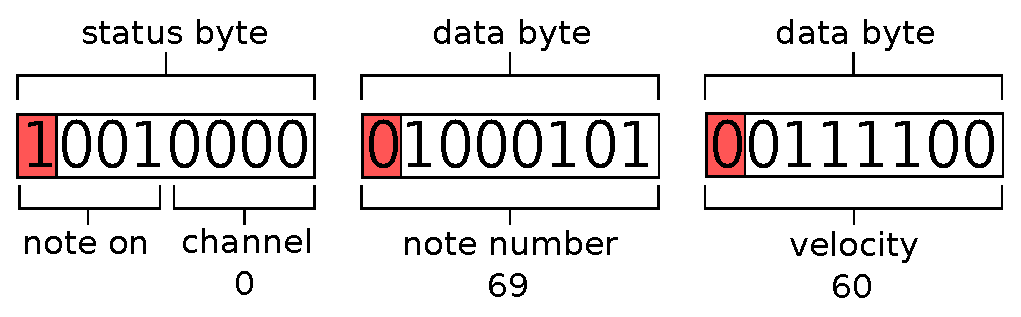
\includegraphics[width=0.7\columnwidth]{TeX_files/midi_message.eps}
    \caption{Struttura di un messaggio MIDI di tipo \textit{note on},
    	     con note number 69 e velocity 60. In rosso è evidenziato
             il bit più significativo.}
\end{figure}

Ai fini del progetto, verranno gestiti solamente i messaggi di \textbf{note on} e \textbf{note off} sul canale '0', mentre
ogni altro tipo di messaggio sarà ignorato.
Ogni messaggio di \textit{note on} viene trasmesso nel momento in cui una certa nota deve essere suonata e contiene due data byte: 
il primo, il \textbf{note number}, identifica la nota da riprodurre, mentre il secondo, detto \textbf{velocity}, fornisce un'informazione
sull'intensità con cui la nota viene suonata. Il suo status byte è del tipo
\textit{1001xxxx} dove \textit{xxxx} sta ad indicare il canale del
messaggio.
Il messaggio note off è analogo e viene trasmesso quando si vuole
interrompere la riproduzione di una certa nota, e il suo status byte
ha il formato \textit{1000xxxx}.
Un altro modo di interrompere la nota (citare standard) è quello di mandare
un messaggio \textit{note on} con \textit{velocity} impostata a zero.

\section{Physical Layer}
I messaggi MIDI vengono trasmessi in maniera seriale e vengono ricostruiti da un convertitore seriale/parallelo detto \textit{UART}(Universal Asynchronous Receiver-Transmitter).
La comunicazione MIDI segue il protocollo RS-232 e funziona nel seguente modo:
\begin{itemize}
	\item In assenza di comunicazione, la linea dati viene mantenuta al valore logico alto
	\item Per compiere una trasmissione, il trasmettitore porta la linea dati al valore logico basso per la durata $T_{bit}$, e questo valore prende il nome di \textbf{start bit}.
	\item I bit da trasmettere vengono inviati in sequenza, in ordine dal bit meno significativo al più significativo; ad ogni bit corrisponde il valore logico alto o basso sulla linea dati per il periodo $T_{bit}$
	\item Alla fine di tramissione la linea dati viene portata al valore logico alto per un tempo di almeno $T_{bit}$, cioè si invia uno \textbf{stop bit}.
\end{itemize}
Il tempo $T_{bit} = \frac{1}{f_{bit}}$ è definito nello standard MIDI imponendo la frequenza di bit a $f_{bit} = \SI{31250}{\hertz}$, detta anche
\textit{baud rate}.
La sequenza di \textit{start bit}, bit di informazione e \textit{stop bit} compongo il \textbf{data frame} del protocollo MIDI.
Si noti che è necessaria a priori la conoscenza del numero di bit da trasmettere perché la comunicazione abbia successo; nello standard MIDI, ad ogni comunicazione viene inviato un byte e quindi 8 bit.
Il protocollo RS-232 permette anche l'aggiunta di un secondo stop bit e di un \textit{parity bit} per il controllo degli errori, tuttavia questi non sono usati nella comunicazione MIDI.
A differenza del protocollo RS-232 i valori logici alti sono segnalati dallo scorrere di una corrente di $\SI{5}{\milli\ampere}$ invece che dalla presenza di un voltaggio positivo.
Il valore logico basso corrisponde all'assenza di corrente.

\section{Il connettore MIDI}
La prima specifica MIDI prevedeva un connettore DIN a 5 pin, 
con un cavo di lunghezza massima di ???, usato per trasmettere
la corrente relativa al bit trasmesso.
Sebbene ancora supportato, questo tipo di connettore fisico è stato
soppiantato con l'avvento del protocollo USB e del relativo connettore,
universalmente supportato dai moderni sintetizzatore come mezzo fisico
di trasmissione per i messaggi MIDI.

\section{Il MIDI tuning standard}
Ad ogni \textit{note number} del protocollo MIDI viene associata una frequenza determinata dal MIDI tuning standard (MTS).
Date due frequenze $f_2 > f_1$ si dice che distano un'\textit{ottava} se
vale la relazione $f_2 = 2 \cdot f_1$.
Si suddivide ogni ottava in 12 note equidistanziate secondo una progressione geometrica, per cui per ogni nota di frequenza $f$ vale

\[
fs^{12} = 2f 
\]

Da cui si ricava la ragione $s=2^{\frac{1}{12}}$ della progressione geometrica. Moltiplicando una frequenza per $s$ si ottiene la frequenza della nota successiva.
Fissando convenzionalmente la frequenza della nota numero 69 a $ \SI{440}{\hertz}$, si ottiene la corrispondenza tra
il note number $i$ e la frequenza $f$ associata:

\[
f = \SI{440}{\hertz} \cdot s^{i-69}
\]

Dal punto di vista musicale, ogni ottava contiene 12 note, e queste
si ripetono più acute o più gravi passando all'ottava successiva o precedente.
Alla frequenza di \SI{440}{\hertz} si associa convenzionalmente
il "la" da concerto, con cui si accordano gli strumenti di un'orchestra.



\chapter{La scheda Nexys4 DDR}

\begin{figure}[h!]
	\centering
	\def\svgwidth{\columnwidth}
	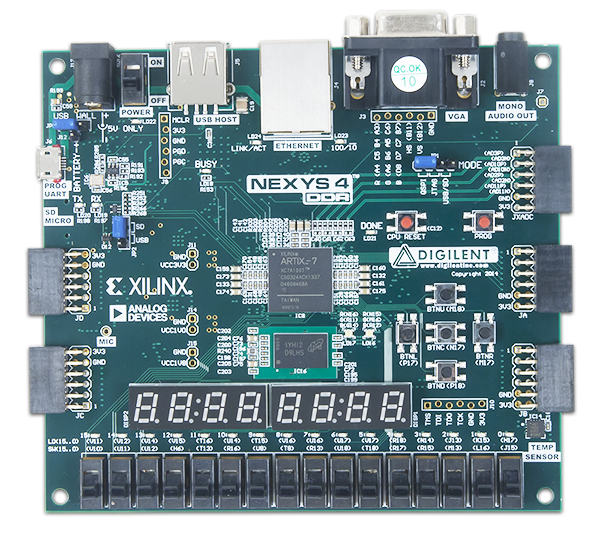
\includegraphics[width=0.6\columnwidth]{TeX_files/nexys4_ddr.png}
    \caption{Scheda Digilent Nexys4 DDR.}
\end{figure}

L'hardware utilizzato per il progetto consiste in una scheda Nexys4 DDR.
Il nucleo della scheda è costituito da un FPGA Xilinx Artix 7 XC7A100T.
Attorno ad esso sono collegati vari connettori, sensori e pulsanti\cite{nexys4referencemanual}.

Per la realizzazione del sintetizzatore si farà uso dei seguenti componenti:
\begin{itemize}
    \item \textbf{Bridge USB-UART} Il bridge USB<->UART permette la lettura
          dei messaggi MIDI, inviati dal computer attraverso la porta seriale
    \item \textbf{Mono Audio Output} Un connettore audio monofonico di tipo minijack 
          viene usato per emettere il suono.
    \item \textbf{Clock Crystal} Il cristallo che fornisce un clock di \SI{100}{\mega\hertz}
          alla FPGA e alla scheda.
\end{itemize}

L'output fornito dal jack audio viene generato attraverso un convertitore analogico/digitale,
costituito da un filtro passa-basso a cui viene fornito in ingresso il segnale
da generare in codifica PWM.

Il filtro passabasso è un filtro di Butterworth del quarto ordine, la cui risposta
in frequenza è rappresentata nella \cref{fig:freq_resp}
\begin{figure}[h!]
	\centering
	\def\svgwidth{\columnwidth}
	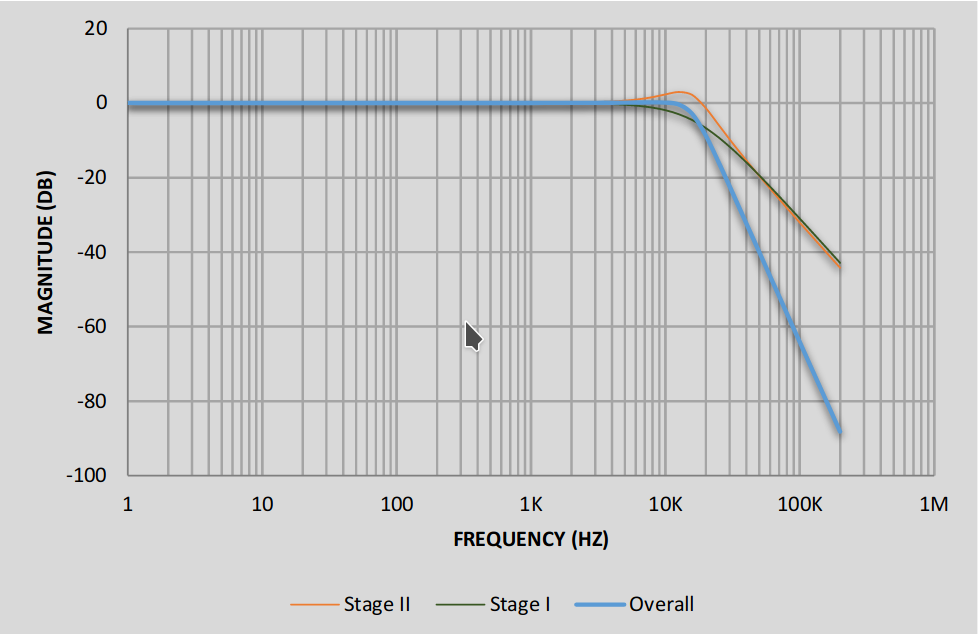
\includegraphics[width=0.6\columnwidth]{TeX_files/freq_response.png}
    \caption{Risposta in frequenza del filtro passa-basso prima dell'uscita audio}
    \label{fig:freq_resp}
\end{figure}

\section{FPGA}
Un Field-programmable Gate Array (FPGA) è un circuito digitale integrato
capace di implementare le più svariate funzioni in modo programmatico:
può essere utilizzato per la fase di prototipazione di Application-specific
Integrated Circuits (ASIC), oppure per sostituirli nel caso in cui i costi
di integrazione di una FPGA nel progetto siano minori dei costi di sviluppo
e realizzazione dell'ASIC (che di solito sono più vantaggiosi per volumi
di produzione molto grandi).
Un FPGA, data la sua natura generale, offre performance inferiori sia
in consumi che in prestazioni rispetto ad un ASIC, ma ha come vantaggio
la riprogrammabilità (anche una volta integrato nel progetto), che
è invece impossibile con un circuito integrato specifico. 
Un altro uso che si va affermando negli ultimi anni è l'utilizzo dei
FPGA come acceleratori software, ad esempio per applicazioni di 
trading finanziaro e intelligenza artificiale. (citare?)

\subsection{Struttura di un FPGA}
Una FPGA ha una struttura regolare e contiene:
\begin{itemize}
    \item \textbf{configurable logic blocks}: in breve \textbf{CLB}, blocchi
            logici configurabili che permettono di realizzare funzioni
            logiche arbitrarie
    \item \textbf{configurable routing}: i blocchi logici sono collegati
          attraverso delle connessioni a loro volta configurabili,
          rendendo possibile creare funzioni logiche a un maggior numero
          di ingressi e più complesse
\end{itemize}

Oltre a queste due componenti fondamentali, un FPGA contiente altri
componenti necessari al suo funzionamento e interfacciamento con
circuiti esterni.
Il FPGA utilizzato dalla scheda Nexys 4 DDR è uno Xilinx Artix 7 XC7A100T
e contiene svariati blocchi\cite{artix7overview}, tra cui:

\begin{itemize}
    \item \textbf{I/O blocks}: blocchi di input e output,
           permettono al FPGA di interfacciarsi con l'esterno
    \item \textbf{DSP blocks}: blocchi che rendono più efficiente in termini
           di risorse l'implementazione di sommatori e moltiplicatori
    \item \textbf{Memory blocks}: è possibile trovare anche blocchi di
           memoria all'interno di un FPGA
    \item \textbf{Clock Management Tiles}: oltre a contenere la circuiteria
            necessaria per la gestione e propagazione del segnale di clock,
            permettono operazioni avanzate sul segnale di clock come la
            generazione di clock a frequenze diverse o di clock sfasati
    \item \textbf{Dedicated blocks}: Blocchi contenenti funzionalità avanzate,
            come ad esempio l'interfaccia PCI Express e blocchi di I/O ad alta
            velocità
\end{itemize}

Esso contiene 101440 logic elements (i blocchi elementari di un CLB), e sei
clock management tiles (CMT) con phase-locked loop.
Di importanza per il progetto trattato sono i 240 DSP slices, 
data la presenza di molti sommatori all'interno del design,
 e i 4860 Kbits di Block Ram (BRAM) che vengono impiegati in fase di 
sintesi per memorizzare sia la forma d'onda campionata che
le frequency tuning words impiegate nella digital direct synthesis.

\subsection{Struttura di un CLB}
Il CLB è la macrostruttura fondamentale di una FPGA.
I circuiti elementari all'interno di un CLB sono i logic elements, che implementano
con una look-up table (LUT) una funzione logica a 5 o 6 ingressi.
Alcune LUT sono utilizzabili anche come elementi di sola memorizzazione.
Ogni logic element contiene anche un elemento di memoria in cui poter memorizzare il risultato
dell'operazione, configurabile sia come flip-flop che come latch.
 Quattro logic elements, insieme a dei multiplexer e alla catena
del carry formano uno logic slice.
Due slice combinati formano quindi un CLB nella sua interezza.

\begin{figure}[hb]
	\centering
	\def\svgwidth{\columnwidth}
	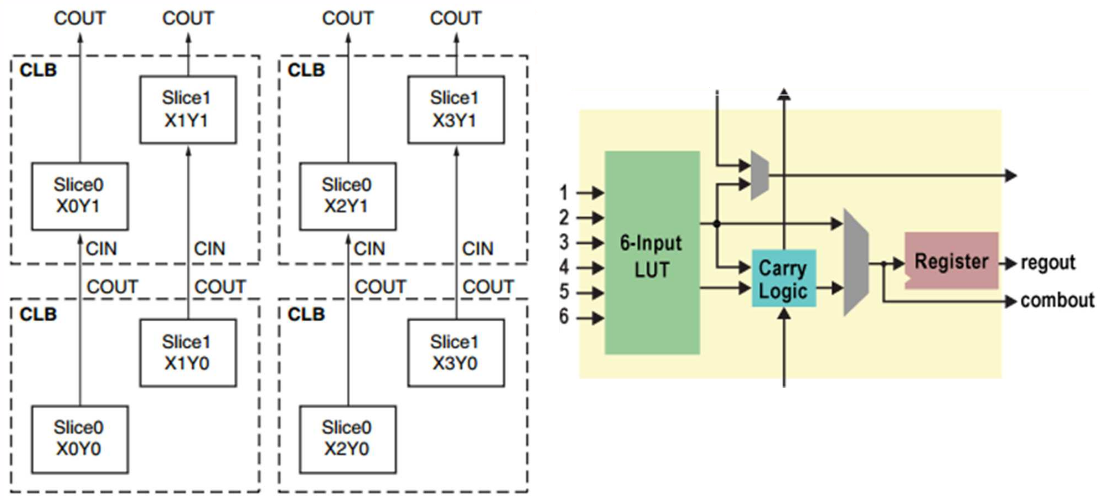
\includegraphics[width=0.8\columnwidth]{TeX_files/CLB.png}
    \caption{Struttura gerarchica di una FPGA: a sinistra l'insieme di più CLB,
    a destra la struttura di un singolo logic element}
\end{figure}

\section{Programmazione di un FPGA}
La programmazione di un FPGA avviene a livello fisico attraverso
la scrittura di una SRAM che indica come vanno configurati i blocchi
logici e le interconnessioni presenti nell'IC.

A livello di sviluppo si utilizzano linguaggi di descrizione dell'hardware
(HDL) come VHDL e Verilog, che nascondono in gran parte la complessità
dell'FPGA.

Il codice sorgente viene processato da un programma di sintesi che compie
all'incirca le seguenti operazioni:

\begin{itemize}
    \item \textbf{Creazione del netlist}: il codice viene convertito in una
          netlist composta da componenti ad alto livello (come sommatori,
          multiplexer, registri ecc..) che tuttavia non combacia
          con la struttura fisica della FPGA
    \item \textbf{Place and Route}: la netlist viene mappata fisicamente sui
          componenti della FPGA
    \item \textbf{Bitstream Generation}: Il risultato del Place and Route viene
          convertito in una serie di bit che vengono poi scritti sulla SRAM
          del FPGA in fase di programmazione
\end{itemize}

\section{Vincoli temporali}
In fase di progetto e di sviluppo il design può essere simulato e analizzato
ben prima di passare alla programmazione della scheda.
Un passo particolarmente importante è l'analisi dei tempi di propagazione:
successivamente al place and route, è possibile calcolare il tempo di propagazione
del segnale attraverso i circuiti del FPGA. Nel caso in cui siano presenti
delle route con un tempo di propagazione troppo lungo, sarà necessario
intervenire a livello del design o addirittura manualmente nel posizionamento
dei blocchi sulla FPGA.
Questo passo viene detto soddisfacimento dei vincoli temporali (timing constraints).

Il periodo di clock utilizzato nel progetto è di 
$T_{clk} = \SI{10}{\nano\second}$, che è il minore possibile sulla scheda
Nexys4 DDR.
In un collegamento tra due elementi sequenziali (ad esempio flip-flop)
il tempo di propagazione dell'uscita del primo elemento all'entrata del
secondo elemento non può quindi superare il periodo di clock.
Ordinando tutte le route per tempo di propagazione decrescente e
considerando quella avente tempo $t_{max}$ di propagazione maggiore, si definisce
il \textbf{Worst Negative Slack} (WNS) come:

\[
\textrm{WNS} = T_{clk} - t_{max}
\] 

Quando questo diventa negativo vuol dire che i timing constraints non
sono rispettati. 

\DeclarePairedDelimiter\floor{\lfloor}{\rfloor}

\chapter{Sintesi digitale del segnale}

TODO: descrivere brevemente la catena del segnale con un grafico
parlare di teorema di campionamento Nyquist?

\section{Sintesi digital diretta}
La sintesi digitale diretta (Direct Digital Synthesis, Direct Digital Frequency Synthesis, DDS) permette di generare un segnale periodico di frequenza programmabile attraverso un sistema digitale.

In termini formali, si vuole generare un segnale $x(t)$ periodico di periodo ??? di frequenza angolare (?) $2\pi f$, ampiezza tra -1 e 1??? fase iniziale nulla.
..dire come si riconduce un segnale di periodo $T$ generico a un segnale
periodico di periodo $2\pi f$ 
Un sistema di DDS si compone di due blocchi: il \textbf{phase accumulator} (PA), responsabile di generare la fase del segnale a una determinata frequenza, e il \textbf{phase to amplitude convereter} (PAC), che a partire dalla fase ottiene l'ampiezza del segnale.

In un sistema a campioni, il PAC si avvale di una ROM di $2^{\code{M}}$ parole contenente il segnale campionato a \code{b} bit.
Altre tecniche possibili per generare i campioni sono algoritmiche (ad esempio l'algoritmo CORDIC per generare segnali sinusoidali) [TODO]

Il \textit{phase accumulator} è un registro a $\code{N}$ bit il cui valore rappresenta la frazione del periodo $[0, 2\pi]$ in notazione
fixed point. Ad ogni fronte di salita del clock il valore $\code{F}$ del registro viene incrementato di un valore pari alla \textit{frequency tuning word},
sempre di $\code{N}$ bit, che è in relazione biunivoca con la frequenza $f$ desiderata.

Si ricorda che la fase del segnale $x(t)$ al tempo $t$ è definita come
\[
\phi(t) = 2\pi f t
\]

Nella sintesi digitale, la fase al tempo $t$ si ottiene dal registro di fase secondo quando descritto prima:
\[
\phi = \frac{2\pi \code{F}}{2^\code{N}}
\]

Essendo \code{F} a precisione finita, si avrà un errore (TODO: basso) sulla precisione della fase del segnale.

Sommando la frequency tuning word al valore del registro di fase \code{F} si ottiene il nuovo valore \code{F'},
e poiché l'addizione avviene ad ogni periodo di clock $T_{clk}$ i valori della fase del segnale corrispondenti sono
$\phi(t)$ e $\phi(t + T_{clk})$.
Si può quindi ricavare la \code{FTW} imponendo:
\[
\code{FTW} = \code{F'} - \code{F} = 
\floor{\frac{2^\code{N}}{2\pi}\phi(t+T_{clk}) - \frac{2^\code{N}}{2\pi}\phi(t)}
= \floor{2^\code{N} f T_{clk}} = \floor{2^\code{N} \frac{f}{f_{clk}}}
\]

Dove $\floor{\cdot}$ indica la parte intera.

La frequenza effettiva $f_{o}$ del segnale risultante dalla DDS è dunque
\[
f_{o} = \frac{\phi(T_{clk}) - \phi(0)}{2\pi T_{clk}} = \frac{2\pi \code{FTW}}{2^\code{N} 2 \pi T_{clk}} = \frac{\code{FTW}}{2^N} f_{clk}
\]
in generale diversa dalla $f$ desiderata per via dell'errore di troncamento della fase.

... non serve fase iniziale nulla: il registro contenente la ftw permette
di avere fase iniziale non nulla. Parlare della precisione del 
phase accumulator ...
...dire secondo quali condizioni valgono le formule: ad es f minore fclock/2, k < p...

...usare approssimazioni per stimare errore, magari grafico..

Il PAC genera un nuovo campione alla frequenza di campionamento $f_s$.
L'udito umano è capace di percepire frequenza fino a circa $\SI{21}{\kilo\hertz}$, per cui è necessaria una frequenza di campionamento di almeno $\SI{42000}{\hertz}$.

Per ricostruire il segnale in uscita il campione viene processato da un convertitore digitale/analogico, e il segnale a tempo continuo risultante viene infine processato da un filtro passa-basso.

\section{Conversione D/A attraverso PWM}
Per portare il segnale discreto generato attraverso la DDS al dominio analogico si fa uso di una tecnica di modulazione detta \textbf{pulse-width modulation} (PWM).

Per comprendere il funzionamento della PWM si consideri un semplice esempio: si voglia rappresentare un segnale costante $x(t) \equiv x_0$ con $x_0 \in [0, x_{max}]$

Sia quindi $x_{pwm}(t)$ un'onda quadra di ampiezza $x_{max}$, di periodo $T$ e di duty cycle $d=\frac{x0}{x_{max}}$, $d \le 1$:
\[
x_{pwm}(t) = \begin{cases}
	x_{max} & \text{se}\ kT \le t < (k+d)T \\
	0 & \text{se}\ (k+d)T \le t < (k+1)T
\end{cases}
\] 
con $k \in Z$

È noto che questo segnale è sviluppabile in serie di Fourier come: ...

In particolare, il coefficiente $a_0$ è pari alla media del segnale sul periodo, ossia
\[
a_0 = x_{max} \cdot d = x_0
\]

È possibile quindi ricostruire il segnale $x(t)\equiv x_0$ a partire da $x_{pwm}(t)$ passandolo attraverso un filtro passa-basso che rimuova tutte le armoniche diverse da $a_0$.

Nel caso in esame $x(t)$ non sarà costante, ma sarà variabile e rappresenterà la forma d'onda generata dal sistema di sintesi digitale diretta.

Al segnale costante verrà quindi sostituito il segnale a tempo discreto $x(kT), k \in Z$ generato alla frequenza di campionamento $f_s = \frac{1}{T}$ e con valori $0 \leq x(kT) \leq x_{max}$, e in prima approssimazione il segnale $x_{pwm}$ corrispondente sarà
\[
x_{pwm}(t) = \begin{cases}
	x_{max} & \text{se}\ kT \le t < (k + d_k)T \\
	0 & \text{se}\ (k+d_k)T \le t < (k+1)T
\end{cases}
\]
dove $(d_k)_{k \in \mathbb{N}}$ è una sequenza di duty cycle non più costanti ma \textbf{modulati} e dati da
\[
d_k = \frac{x(kT)}{x_{max}}
\]

Tuttavia il segnale PWM è generato digitalmente, quindi supponendo per semplicità $T=1/f_s$ multiplo del periodo di clock $1/f_{clk}$, in un singolo periodo
di campionamento si avrà una successione di $N=\frac{f_{clk}}{f_s}$ impulsi pari a $x_{max}$ (corrispondente ad un valore logico alto) o $0$ (corrispondente a un valore logico basso).
Poiché al fine della modulazione PWM conta solo il valore medio sul periodo, l'ordine degli impulsi non cambia il risultato, anche se cambia la distribuzione delle armoniche nello spettro del segnale.
È quindi possibile rappresentare un numero finito di valori in uscita pari a $N$, e quindi i campioni forniti potranno al massimo avere una risoluzione di $\log_2{N}$ bit.

La modulazione PWM non è lineare e introduce quindi distorsione nel segnale ricostruito.

\newcommand{\blockdiagram}[4]{
	\begin{tikzpicture}[font=\sffamily,>=triangle 45]
         \node [circuit] (item) {};
		
		\matrix[
		matrix of nodes,
		left= of item,
		row sep=\myheight/15,
		nodes={anchor=east}
		] (rightmatr) {
			#3
			\\
		};
		\matrix[
		matrix of nodes,
		right= of item,
		row sep=\myheight/15,
		nodes={anchor=west}
		] (leftmatr) {
			#4
			\\
		};
	
		\foreach \i in {1,...,#1}
			\draw [->] (rightmatr-\i-1) -- (rightmatr-\i-1 -| item.west);
		\foreach \i in {1,...,#2}
			\draw [<-] (leftmatr-\i-1) -- (leftmatr-\i-1 -| item.east);
	\end{tikzpicture}
}


\chapter{Architettura ed implementazione}

L'architettura da sintetizzare su FPGA è stata sviluppata utilizzando il linguaggio VHDL, facendo
ampiamente uso di molte funzionalità della versione VHDL-2008.
Il progetto è stato sintetizzato usando il software Vivado 2019.1 della Xilinx e simulato usando il compilatore/simulatore open-source GHDL.

Dal punto di vista architetturale si può considerare il progetto come composto da due macro-blocchi indipendenti: uno che si occupa di gestire i segnali MIDI dati in input al sintetizzatore e uno che si occupa di generare il segnale audio in uscita.

Le due componenti sono implementate in logica sincrona e sono collegate da una lookup table che memorizza le note attive. Alla ricezione di un evento MIDI \textit{note on} il bit corrispondente alla nota nella LUT viene portato al valore logico alto, e al seguente istante di campionamento la componente che genera il segnale di output userà questo valore per determinare se suonare o meno la nota.

\section{Scelta dei parametri di progetto}
Mentre la frequenza di clock $f_{clk} = \SI{100}{\mega\hertz}$ e 
la frequenza di campionamento minima $f_{s,min} = 2 \cdot \SI{21000}{\hertz}$
sono date, non sono note a priori i seguenti parametri:
\begin{itemize}
    \item \textbf{\code{b}}: Numero di bit usati per quantizzare la forma d'onda
    \item \textbf{\code{N}}: Numero di bit usati per il registro di fase nel phase accumulator
    \item \textbf{\code{M}}: Numero di bit presi tra i primi bit del registro di fase e usati per indirizzare i campioni
\end{itemize}

Utilizzando i vincoli imposti dalla conversione D/A in PWM, si 
ottiene il numero massimo di bit del quantizzatore imponendo che

\[
\code{b} < \Big \lceil \log_{2}{\frac{f_{clk}}{f_{s,min}}} \Big \rceil = 12
\]

Conviene quindi massimizzare \code{b} per avere una minore errore di quantizzazione,
e allo stesso tempo massimizzare il più possibile $f_s$, scegliendola per comodità
come sottomutiplo della frequenza di clock.
Si ottiene così $\code{b} = 11$ e $f_s = \SI{48828}{\hertz}$

Nella seguente tabella sono riportati i valori dei parametri e, in aggiunta, i relativi
nomi all'interno del progetto VHDL.

\begin{tabular}{| c | c | m{10em} | l | }
 \hline
 \textbf{Parametro} & \textbf{Valore} & \textbf{Descrizione} & \textbf{VHDL constant}\\
 \hline
 $f_{clk}$  & \SI{100}{\mega \hertz} & frequenza di clock del FPGA  & \code{clock\_frequency}\\
 \hline
 $f_s$ &  \SI{48828}{\hertz} & frequenza di campionamento & \code{sampling\_frequency}\\
 \hline
 \code{b} & 11 & numero di bit dei campioni & \code{sample\_bits}\\
 \hline
 \code{N} & 32 & numero di bit del registro di fase e della frequency tuning word & \code{phase\_bits}\\
 \hline
 \code{M} & 13  & numero di bit degli indirizzi dei campioni & \code{address\_bits}\\
 \hline
\end{tabular}

\section{Componenti fondamentali}
I seguenti blocchi fondamentali corrispondono in VHDL al costrutto di \textit{entity} e veranno analizzati dettagliatamente in seguito:

\begin{itemize}
    \item \hyperref[sec:counter]{\code{counter\_impulse\_generator}} Un contatore con frequenza di reset variabile, viene
    usato principalmente per la sincronizzazione temporale tra diversi componenti
    \item \hyperref[sec:lowhigh]{\code{low\_to\_high\_detector}} Componente ausiliario che trasforma la variazione
    del segnale in ingresso dal valore logico basso a quello alto in un impulso della durata di un ciclo
    di clock
    \item \hyperref[sec:uart]{\code{uart}} Si occupa della ricezione seriale a 31250 baud secondo le specifiche MIDI
    \item \hyperref[sec:mididec]{\code{midi\_decoder}}  State machine che codifica i byte ricevuti dal blocco uart in eventi MIDI; gestisce solamente gli eventi note on/off
    mentre scarta tutti gli altri eventi MIDI.
    \item \hyperref[sec:noteslut]{\code{active\_notes\_lut}} Tabella di lookup contenente 128 valori booleani che indicano l'attivazione di una nota
    \item \hyperref[sec:phaseaccumulator]{\code{phase\_accumulator}} Opera l'accumulazione di fase per la DDS
    \item \hyperref[sec:pwmencoder]{\code{pwm\_encoder}} Genera la modulazione PWM corrispondente in uscita
    a partire da un campione fornito in entrata
    \item \hyperref[sec:rom]{rom} Package generico che rappresenta una read-only memory.
    \item \hyperref[sec:synthengine]{\code{synth\_engine}} Cuore del sintetizzatore, provvede alla DDS a partire dai valori presenti in active\_notes\_lut, alla phase-to-amplitude conversion attraverso una ROM e al mixing.
    \item \code{synth\_top} Entità top del progetto, cioè che contiene tutte le altre entity e le istanzia nel modo corretto, impostando le frequenze di lavoro dei componenti.
\end{itemize}

\section{Contatore Generico}
\label{sec:counter}

\begin{center}
	\blockdiagram{2}{2}{
		i\_clock \\ i\_rst
	}{
	    o\_signal \\ o\_counter
    }
\end{center}
L'entity \code{counter\_impulse\_generator} implementa un contatore generico.
Facendo uso dei parametri generici del VHDL è possibile impostare per ogni istanza
del componente una diversa frequenza di reset.
Il contatore utilizza un registro che viene incrementato ad ogni ciclo di clock
e la sua dimensione in bit è calcolata automaticamente a partire dalle frequenze
di reset e di clock. Il valore del registro è esposto alla porta \code{o\_counter}.
Al reset del contatore il segnale di output \code{o\_signal} viene portato al valore
logico alto per un ciclo di clock.
Si utilizza questo segnale per abilitare i componenti che devono
effettuare operazioni a una frequenza inferiore alla frequenza di clock:
ad esempio per pilotare il processo di campionamento si fa uso di un contatore
avente frequenza di reset uguale alla frequenza di campionamento \code{sampling\_frequency}.

\section{Blocco UART}
\label{sec:uart}

%\begin{lumos}
%	\luminput{
%		i\_clock \\
%		i\_serial\_input \\
%	}
%	\lumoutput{
%		o\_data\\
%		o\_data\_available
%	}
%\end{lumos}

\begin{center}
	\blockdiagram{2}{2}{
		i\_clock \\ i\_serial\_input
	}{
	    o\_data \\ o\_data\_available
    }
\end{center}

Il blocco uart è composto da una finite state machine (fsm) e uno shift register da 9 bit, contenente inizialmente i valori '0' tranne per il bit più significativo che è posto a '1' e funge da sentinella. La lettura della linea dati avviene periodicamente alla frequenza $f = \frac{1}{T_{bit}} = 31250 \si{Hz}$; alla ricezione dello start bit, la fsm entra nello stato di ricezione e si fa avanzare lo shift register leggendo il valore presente sulla linea nel bit più significativo, facendo contemporaneamente slittare gli altri verso destra.
A lettura ultimata, lo shift register è avanzato di 8 posizioni e il bit meno significativo dello shift register contiene il bit sentinella; con questo si indica la fine della trasmissione.

\section{MIDI decoder}
\label{sec:mididec}

\begin{center}
	\blockdiagram{3}{2}{
		i\_clock \\
		i\_enable \\
		i\_data \\
	}{
	    o\_message \\
	    o\_message\_available
    }
\end{center}
Il decoder MIDI si occupa di leggere i byte provenienti dal convertitore seriale/parallelo e di convertirli in messaggi MIDI.
In realtà il componente è molto semplificato in quanto interpreta solo i messaggi di note on e note off, mentre scarta ogni altro messaggio MIDI.
Il blocco è implementato attraverso una fsm; quando l'input \code{i\_enable} viene mantenuto alto per un ciclo di clock, la state machine avanza leggendo il byte \code{i\_data} in input.
Quando il messaggio è stato completamente decodificato, l'output \code{o\_message\_available} assume un valore logico alto e il messaggio MIDI è disponibile in uscita al blocco.

\section{Low to High detector}
\label{sec:lowhigh}

\begin{center}
	\blockdiagram{2}{1}{
		i\_clock \\ i\_signal
	}{
	    o\_detected
    }
\end{center}

Quando l'entrata \code{i\_signal} passa dal valore logico basso a quello alto,
\code{o\_detected} assume il valore logico alto per un singolo ciclo di clock.
Un esempio di utilizzo di questo componente è la connessione tra i componenti
\hyperref[sec:uart]{uart} e \hyperref[sec:mididec]{midi\_decoder}: il blocco
\code{midi\_decoder} avanza la macchina a stati leggendo dall'ingresso quando
la porta \code{i\_enable} si trova al valore logico alto. Se questa fosse
collegata direttamente all'uscita \code{o\_data\_available} del blocco \code{uart},
lo stesso byte verrebbe processato più volte non permettendo una decodifica
corretta. Si intermezza questa connessione con un componente \code{low\_to\_high\_detector}
cosicché alla presenza di un nuovo byte il decoder midi venga abilitato solo per
un ciclo di clock.
Nonostante la sua semplicità questa entity permette di semplificare altre situazioni
in cui questo avviene all'interno del progetto.

\section{Active Notes LUT}
\label{sec:noteslut}

\begin{center}
	\blockdiagram{3}{1}{
		i\_clock \\
		i\_enable \\
		i\_message \\
	}{
		o\_active\_notes\_reg
	}
\end{center}
Quando il segnale \code{i\_enable} è alto per un ciclo di clock, il valore del messaggio midi in input viene letto e il registro \code{o\_active\_notes\_reg} viene modificato in modo che il bit in posizione corrispondente alla nota sia 1 o 0 a seconda del contenuto del messaggio.

\section{Accumulatore di Fase}
\label{sec:phaseaccumulator}

\begin{center}
	\blockdiagram{3}{1}{
		i\_clock \\
		i\_rst\_sync \\
		i\_ftw \\
	}{
		o\_phase\_reg
	}
\end{center}
L'accumulatore di fase implementa il registro di fase utilizzato nella DDS.
La grandezza del registro è impostabile attraverso il parametro generico \code{phase\_bits}.
È possibile il reset sincrono del registro impostando al valore logico alto il segnale \code{i\_rst\_sync}.

\section{PWM Encoder}
\label{sec:pwmencoder}

\begin{center}
	\blockdiagram{2}{1}{
		i\_clock \\
		i\_sample
	}{
		o\_pwm\_signal
	}
\end{center}
Il \code{pwm\_encoder} funziona nel seguente modo: all'interno dell'entity
è istanziato un registro contatore che viene incrementato ad ogni ciclo di clock
e ritorna nullo dopo $K$ cicli di clock, dove
\[
  K = \floor*{\frac{T_s}{T_{clk}}} = 2048
\]
uguale ai $2^b$ possibili valori che può assumere un campione.
Si ha quindi
\[
  K = 2^b = \code{i\_sample\_max} + 1
\]
Dopo $T_{clk}K \approx T_s$ il contatore si riazzera e si ha un nuovo campione
in ingresso.
Il valore del campione \code{i\_sample} viene confrontato con quello del registro; se
questo è maggiore del valore del contatore, l'uscita viene portata in alta impedenza,
mentre se questo è minore l'uscita viene portata a zero.
L'uscita \code{o\_pwm\_signal} pilota l'uscita audio monofonica e
viene posta ad alta impedenza invece che al valore logico alto per permettere
al circuito di gestire autonomamente il voltaggio di uscita.
La frazione di tempo per cui \code{o\_pwm\_signal} rimane in alta impedenza
in un intervallo di campionamento è di
\[
\frac{T_{clk}\code{i\_sample}}{K T_{clk}} = 
\frac{\code{i\_sample}}{\code{i\_sample\_max}+1}
\]

Detto $v_{gain}$ il voltaggio massimo fornito al filtro passa-basso,
si vede facilmente che la media sul periodo del segnale è
\[
v_{gain} \cdot\frac{\code{i\_sample}}{\code{i\_sample\_max}+1}
 \approx v_{gain} \cdot \frac{\code{i\_sample}}{2^\code{b}} \approx v_{gain}s(k T_s)
\]
Dove si è usata all'ultimo passaggio l'\cref{eq:quantization}, ignorando gli errori
dovuti alla DDS e alla quantizzazione.
È chiaro quindi che il segnale dato in ingresso viene amplificato e
ricostruito dal filtro in base a quanto detto nella \cref{sec:quantizationrom}.

\begin{figure}
	\centering
	\def\svgwidth{\columnwidth}
	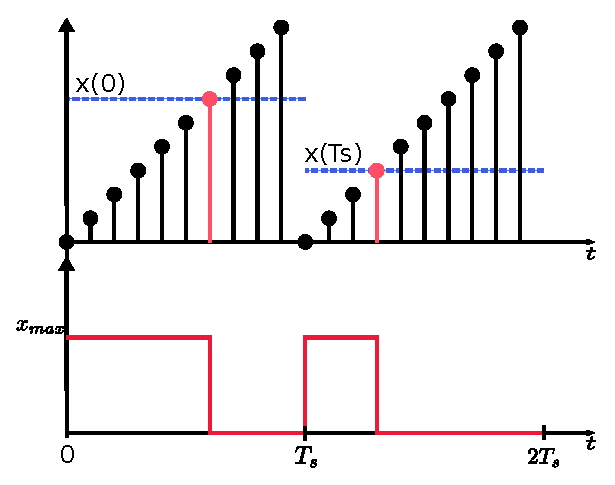
\includegraphics[width=0.7\columnwidth]{TeX_files/pwm_ramp.eps}
	\caption{Esempio di PWM: nel grafico sopra è riportato il valore del campione $s(kT_s)$ - tratteggiato in blu - che viene comparato al contatore.
	Quando il contatore supera il valore di $s(kT_s)$, \code{o\_pwm\_signal} passa da $x_{max}$ a $0$. }
\end{figure}

\section{Componente ROM}
\label{sec:rom}
Le ftw e la forma d'onda da riprodurre vengono generate attraverso due
script python e salvate in un file.
Il package generico rom permettere al progetto di avere queste informazioni in fase di sintesi: si specificano i tre parametri \code{word\_bits}, che indica il numero di bit per parola nella memoria, \code{address\_bits}, che indica il numero di bit necessari a indirizzare una parola, e \code{rom\_filename}, che specifica il file testuale da leggere contenente le parole della rom.
Il file deve essere formattato nel seguente modo: ci sono tante righe quanti sono gli indirizzi della memoria, ogni riga è una stringa binaria
di lunghezza fissa e rappresenta la parola memorizzata.
Gli indirizzi partono da 0 (prima riga) e aumentano di un unità ad ogni riga.
È possibile leggere dalla ROM usando la funzione \code{read\_at}, specificando come argomento l'indirizzo desiderato.

\begin{minted}{VHDL}
package rom is
  generic (
    word_bits: positive;
    address_bits: positive;
    rom_filename: string
  );
  subtype word_type is std_logic_vector(word_bits-1 downto 0);
  impure function read_at(
     address: in integer range 0 to 2**address_bits-1
  ) return word_type;
end package rom;
\end{minted}

\section{Synth Engine}
\label{sec:synthengine}

\begin{center}
	\blockdiagram{2}{2}{
		i\_clock \\
		i\_active\_notes
	}{
		o\_sample \\
		o\_sample\_ready
	}
\end{center}


Il componente principale del sintetizzatore ha accesso alla LUT contenenti le note attive e genera ad ogni periodo di campionamento
un campione del segnale.

Attraverso il package \hyperref[sec:rom]{rom} vengono rese disponibili a questo componente la forma d'onda campionata e le frequency
tuning word corrispondenti ad ogni possibile nota suonata.
Attraverso il costrutto \code{for .. generate} vengono generati 128 accumulatori di fase indipendenti. Ad ognuno di questi viene accoppiata
una entity che ne esegue il reset quando una nota passa dal valore logico basso a quello alto nella LUT
(si noti l'utilizzo del componente \hyperref[sec:lowhigh]{\code{low\_to\_high\_detector}}).
\begin{minted}{VHDL}
oscillators:
for i in 0 to MAX_MIDI_NOTE_NUMBER generate
    signal ftw: std_logic_vector(phase_bits-1 downto 0);
    signal reset_signal: std_logic := '0';
begin
    ftw <= phase_rom.read_at(i);
    reset_generator: entity work.low_to_high_detector
    port map (
        i_clock => i_clock,
        i_signal => i_active_notes(i),
        o_detected => reset_signal
    );
    accumulator: entity work.phase_accumulator
    generic map (
        clock_frequency => clock_frequency,
        phase_bits => phase_bits
    )
    port map (
        i_clock => i_clock,
        i_rst_sync => reset_signal,
        i_ftw => ftw,
        o_phase_reg => phase_vec(i)
    );
end generate oscillators;
\end{minted}

Il campione viene fornito alla porta \code{o\_sample} e viene generato attraverso un processo di mixing.
Il mixing consiste nel seguente processo, ripetuto per ogni valore della LUT delle note attive:
\begin{itemize}
    \item Se la nota è attiva, si carica il valore campionato della forma d'onda ad essa relativa:
          il valore campionato viene ottenuto dalla ROM dei campioni, usando come indice
          i primi \code{M} bit dell'accumulatore di fase: infatti questo è il
          \textbf{phase to amplitude converter} (PAC)
    \item Il valore del campione viene sommato su un registro inizialmente nullo
\end{itemize} 

Come verrà chiarito nella \cref{sec:timing_impl}
l'implementazione fa uso di una pipeline a due stadi:
il primo stadio della pipeline provvede alla PAC, mentre il secondo stadio
esegue parallelamente il mixing con il valore ottenuto dallo stadio
precedente.
\begin{figure}[H]
	\centering
	\def\svgwidth{\columnwidth}
	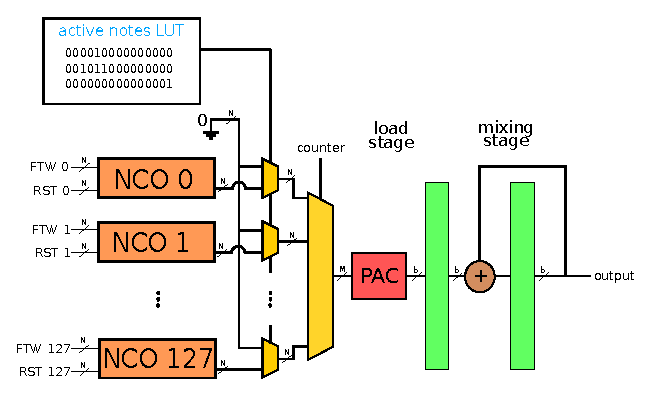
\includegraphics[width=\columnwidth]{TeX_files/synth_engine.eps}
	\caption{Architettura con pipeline a due stadi. Ogni multiplexer
	 in uscita ad un phase accumulator (PA) controlla se la nota è attiva nella LUT; il
     multiplexer principale, comandato da un contatore, carica la pipeline
     con un nuovo campione. Seguono poi lo stadio di PAC (ossia il caricamento del campione dalla ROM) e il mixing.}
\end{figure}

Ogni avanzamento della pipeline viene eseguito in un ciclo di clock,
e in totale sono necessari 129 cicli di clock
(128 per ogni nota, più uno per caricare la pipeline) che vengono eseguiti
appena prima della fine del periodo di campionamento.
Questo avviene all'ultimo ciclo di clock della fase di produzione del
campione, in cui l'output \code{o\_sample\_ready} assume il valore
logico alto per indicare la presenza di un campione.

\section{Difficoltà di implementazione e vincoli temporali}
\label{sec:timing_impl}
Nel corso dello sviluppo del progetto uno dei problemi più difficili da affrontare
è stato quello del rispetto dei vincoli temporali nell'implementazione dell'engine
del sintetizzatore.

Inizialmente questo era stato implementato come un componente asincrono dotato di 
128 ingressi collegati alla LUT delle note attive e 128 ingressi da \code{sample\_bits},
ciascuno collegati direttamente alla memoria dei campioni.
In totale il componente aveva quindi $128+128\cdot11 = 1536$ bit in ingresso, senza contare
il sommatore e i multiplexer necessari alla selezione delle note.
Data la complessità del componente, questo veniva sintetizzato con una lunga catena
di sommatori a due ingressi collegati in cascata; tuttavia le catene di propagazione più lunghe
non rispettavano i vincoli temporali,e si otteneva un WNS di \SI{-1.684}{\nano\second}.

Si è quindi convertito il mixer in un componene sincrono che sommasse ogni campione
ad un ciclo di clock; tuttavia anche in questo caso si otteneva un WNS negativo pari
a \SI{-0.738}{\nano\second}.
Una soluzione si sarebbe potuta ottenere dilatando il tempo tra due operazioni di somma
successive, impostando i parametri di progetti in modo da allentare i timing constraints
su queste path.
Un'altra soluzione simile sarebbe quella di usare un clock diverso per il processo di mixing.
Entrambe le soluzioni tuttavia richiedevano una conoscenza approfondita di Vivado,
e la seconda soluzione necessita della comunicazione tra componenti aventi 
clock diversi, detto \textit{clock domain crossing}, e molto complesso da
implementare.

Notando che la path che non rispettava i vincoli temporali attraversava
il sommatore, si è deciso di rendere l'operazione di caricamento del campione
e quella di somma distinte, formando così l'architettura a pipeline a due stadi descritta prima.

Così facendo il WNS diventa di $\SI{1.911}{\nano \second}$ e i vincoli temporali sono rispettati.

\chapter{Analisi e conclusioni}
Il testing del progetto sulla scheda Nexys4 DDR è stato condotto
attraverso la porta seriale della scheda e mediante l'uso di uno
script Python che automatizzasse la riproduzione di un file MIDI 
(si veda \code{scripts/play\_midi\_file.py}).
Per effettuare il testing funzionale delle varie componenti del progetto
si è fatto uso di \textit{testbenches} scritti in VHDL, che fornissero
un input prefissato a un certo componente per verificarne la risposta,
utilizzando sempre GHDL.
In particolare il testbench descritto nel file
 \code{vhdl/mono\_synth\_engine\_tb.vhd} provvede a testare l'intera
architettura riproducendo una singola nota.
L'uscita del blocco \code{pwm\_encoder} viene quindi salvata ad ogni
ciclo di clock su un file txt, che viene in seguito processato
dallo script \code{scripts/plot\_pwm\_output.py} che lo filtra
digitalmente e visualizza il segnale ricostruito.

L'intero codice del progetto, compresi gli script, i testbench e questa
tesi è disponibile su github \cite{sourcecode}.

Data la complessità computazionale di una simulazione, il testbench
di prova dell'intero progetto può impiegare fino a diversi minuti
per generare un output che realmente avrebbe durata nell'ordine della
decina di millisecondi, tempo insufficiente a fare analisi significative
sul segnale ottenuto.
Si è quindi optato per la simulazione della sintesi DDS, della conversione
in PWM e della ricostruzione del segnale attraverso uno altro script python,
con cui si sono valutate le prestazioni del progetto.

\section{Rapporto Segnale Rumore}
Sia $s(t)$ il segnale da generare e $s'(t)$ il segnale ottenuto
dal processo di sintesi.
Si definisce il \textit{segnale d'errore} $e(t)=s(t)-s'(t)$.
Per valutare la qualità del segnale d'uscita rispetto al segnale di ingresso
si fa uso del cosiddetto \textit{signal to noise ration} (SNR), definito da\cite{tlc}
\begin{equation}
\code{SNR} = \frac{P_s}{P_e}
\end{equation}

Dove $P_s$ e $P_e$ sono la potenza del segnale e del segnale d'errore, che per segnali
reali vale \cite{oppenheim}
\begin{equation}
P_s = \lim_{T\to\infty} \frac{1}{2T}\int_{-T}^{T} s^2(t) dt 
\end{equation}

Per misurare l'SNR si fa spesso l'utilizzo dei decibel, per cui
\begin{equation}
\code{SNR}_{\SI{}{\decibel}} = 10 \log_{10}{\code{SNR}}
\end{equation}

\section{Errore di quantizzazione}
La prima causa di errore nel segnale ricostruito si deve al processo di quantizzazione:
il processo di quantizzazione descritto nella \cref{sec:quantizationrom} si dice
quantizzazione uniforme.
Dato l'intervallo di valori assunti da $x(t)$ pari a $[-x_{max},x_{max}]=[-1,1]$ e il numero di valori
quantizzati $L=2^\code{b}$ (numero di livelli del quantizzatore) si definisce il passo di quantizzazione
\[
\Delta = \frac{2 x_{max}}{L}
\]

Si dimostra che se il segnale $s(t)$ rimane all'interno del range stabilito,
l'errore di quantizzazione ha una potenza pari a\cite{tlc}
\[
P_e = \frac{\Delta^2}{12}
\]

Per il testing di questo progetto si è scelto di utilizzare $A=0.4$ e la forma
d'onda sinusoidale, cosicché
il valore massimo di due segnali sovrapposti non ecceda la soglia di quantizzazione
e non si vada in saturazione con la polifonia a due voci.
Come è noto la potenza di un segnale periodico è uguale alla potenza sul periodo
e nel caso di un segnale $s(t)=A\sin(2\pi ft)$ è pari a
\[
P_s = \frac{A^2}{2}
\]

L'SNR dovuto all'errore di quantizzazione con $\code{b}=11$ è pari a
$\code{SNR}_{\SI{}{\decibel}} = \SI{60}{\decibel}$.

La quantizzazione di un segnale di ampiezza minore di quella massima permessa
dal quantizzatore peggiora la qualità del segnale, infatti se si fosse usato
$A=1$ si sarebbe ottenuto 
$\code{SNR}_{\SI{}{\decibel}} = \SI{67.8}{\decibel}$, andando tuttavia incontro
a problemi overflow in caso di polifonia che annullerebbero la qualità guadagnata.

\section{Errore della PWM}
Come si è ricavato nella \cref{sec:dapwm}, un'onda quadra di duty cycle costante
$d$ e valore tra $0$ e $x_{max}$ produce, dopo un adeguato filtro passabasso,
un segnale costante avente il valore $d x_{max}$.
Quando il duty cycle cambia ad un nuovo valore (ossia alla codifica di un nuovo
campione) si avrà un transitorio prima che la risposta in uscita al filtro
si assesti sul nuovo valore.
Intuitivamente si capisce che la qualità del segnale ricostruito dipende
da quanto velocemente può variare il segnale rispetto alla frequenza
di transizione della PWM.

La condizione per la ricostruzione esatta del segnale PWM si ricava
dall'espressione analitica del suo spettro, molto complessa da ricavare e per
cui si rimanda a \cite{pwmspectrum}.
Date $f_{pwm}=1/T_{pwm}$, definita del periodo del segnale PWM, e la frequenza
 massima del segnale $f_{max}$ si dimostra che
\begin{equation}
f_{pwm} > \pi f_{max}
\end{equation}
è la condizione di ricostruzione del segnale PWM.

Essendo $f_{pwm}=f_s$ nel nostro progetto, si ricava che la frequenza massima del segnale
è di poco più di \SI{15}{\kilo\hertz}, inferiore alla frequenza massima
che ci si era impostati di riprodurre.
Nel caso di segnali aventi contenuto armonico maggiore di questa frequenza,
questo non verrà ricostruito accuratamente; nel caso delle sinusoidi usate
per il testing il problema non si verifica poiché la nota più acuta,
corrispondente al note number 127, ha una frequenza di \SI{12543}{\hertz}.

\section{Errore dovuto alla DDS}
La processo di sintesi digitale diretta introduce due errori: il primo dovuto
alla quantizzazione della fase, il secondo dovuto alla capacità ridotta della
ROM e alla necessità di indirizzarla con i primi \code{M} bit del registro
di fase.
Usando un numero \code{N} di bit elevato per il registro di fase si può
considerare trascurabile l'errore dovuto alla quantizzazione della fase,
mentre non è trascurabile il secondo tipo di errore detto \textbf{errore
di troncamento di fase}.

Data una qualsiasi \code{FTW}, il valore del registro i fase sarà periodico
di un numero di cicli $K$ pari a\cite{analogdevicessec4}
\[
  K = \frac{2^\code{N}}{\textrm{GCD}(\code{FTW}, 2^\code{N})}
\]

Gli ultimi $N-M$ bit del registro di fase saranno anch'essi periodici di un numero
di cicli al massimo uguale a $K$. Essendo questi a determinare l'errore di troncamento
di fase, si evince che il segnale d'errore avrà un andamento periodico 
nel dominio del tempo, a causerà nel dominio della frequenza la presenza
di frequenze spurie.

\begin{figure}[H]
	\centering
	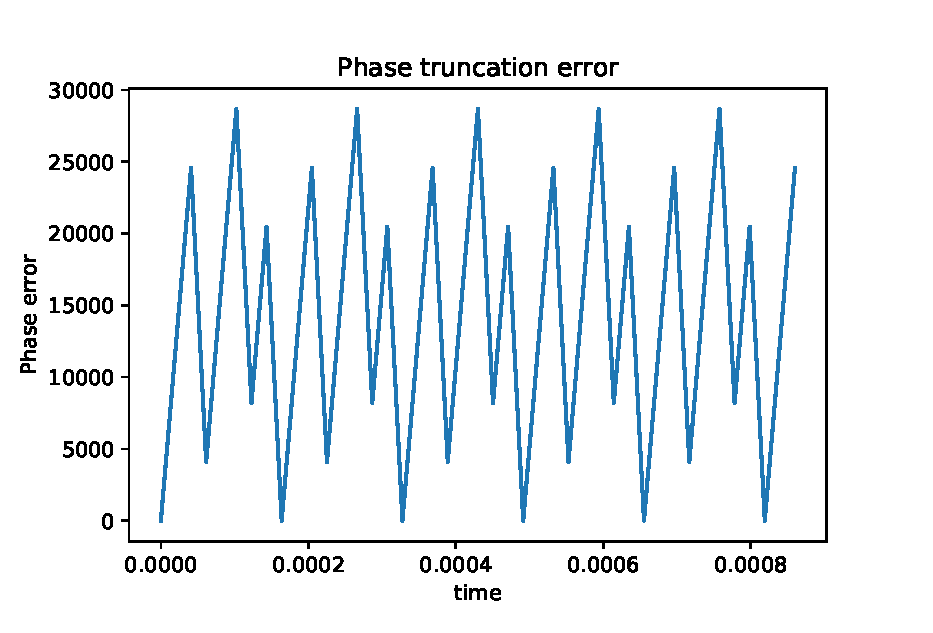
\includegraphics[width=0.85\columnwidth]{TeX_files/phase_truncation_error.eps}
	\caption{Periodicità dell'errore di troncamento di fase corrispondente alla $\code{FTW}=63565$, con $\code{N}=32$ e $\code{M}=17$.}
\end{figure}

In generale quindi l'errore introdotto dalla DDS dipende da $M$ e $N$ ed è diverso per ogni
scelta della \code{FTW}. Si veda \cite{analogdevicessec4} oppure \cite{exactspurs} per una trattazione
più dettagliata della distribuzione e ampiezza delle frequenze spurie nel segnale,
omessa in quanto complessa dal punto di vista matematico.

La riduzione di SNR dovuta alla DDS è stata calcolata, attraverso le simulazioni,
per ogni possibile valore del \textit{note number} ed è riportata in \cref{fig:confronto}.
\begin{figure}[H]
    \begin{minipage}{0.59\columnwidth}
            \centering
            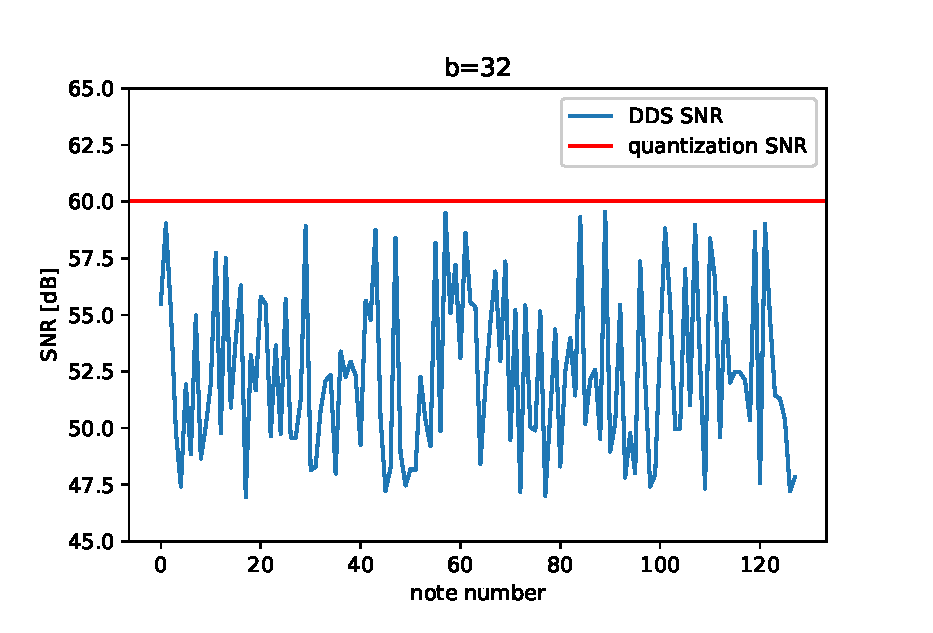
\includegraphics[width=1.0\columnwidth]{TeX_files/dds_snr_32.eps} % first figure itself
        \end{minipage}\hfill
    \begin{minipage}{0.59\columnwidth}
            \centering
            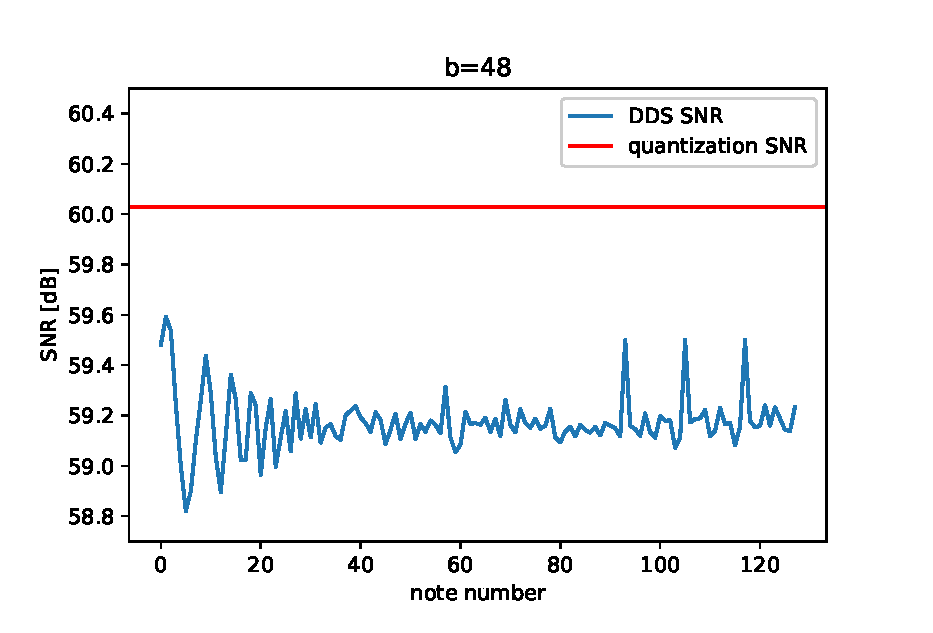
\includegraphics[width=1.0\columnwidth]{TeX_files/dds_snr_48.eps} % second figure itself
    \end{minipage}
    \caption{Confronto dell'SNR dovuto alla DDS con due grandezze diverse del registro di fase.}
    \label{fig:confronto}
\end{figure}

Per $\code{N}=32$ l'SNR decresce fino a circa $\SI{47}{\decibel}$ per alcune
frequency tuning words. Usando una precisione maggiore per il registro di fase
si riesce ad ottenere un SNR al minimo di \SI{58.8}{\decibel}, molto vicino a quello di sola quantizzazione.

\section{Considerazioni finali}
Il sintetizzatore progettato, sebbene funzionante, presenta performance
di SNR non ottimali, dovute alle limitazioni intriseche della pulse-width 
modulation.
La PWM infatti limita il numero di bit di risoluzione del campionatore da un lato
e la frequenza massima rappresentabile dall'altro.
Sarebbe possibile bypassare l'uscita audio monofonica della scheda
e utilizzare un DAC esterno, connesso attraverso le porte PMOD, 
per fornire una qualità audio migliore.
Due esempi sono i componenti PMOD I2S2 e il PMOD AMP2 della Digilent.

La polifonia, essendo implementata con un semplice sommatore in fase 
di mixing, è soggetta ad overflow quando la somma dei campioni supera
la precisione permessa dai \code{b} bits di quantizzazione.
In campo audio questo fenomento viene detto \textit{clipping}.
Di fatto, essendo l'ampiezza del segnale campionato pari a poco meno
della metà del valore massimo rappresentabile, la polifonia è limitata
a due voci, oltre le quali il segnale presenta una degradazione
notevole.

Far rientrare il range del segnale nei limiti con un divisore risolverebbe
il clipping ma degraderebbe la qualità del segnale e causerebbe
sbalzi di volume udibili nel passaggio da una singola nota  a più note
suonate contemporaneamente.

Tecniche più avanzate di compressione dinamica del segnale 
sono molto complesse e al di fuori dello scopo di questa tesi.  

I messaggi MIDI contengono anche l'informazione relativa alla forza
di pressione della nota, detta velocity, come descritto nel \cref{chap:midi}.
Si potrebbe estendere il sintetizzatore per rispettare questa informazione
in due modi differenti:
\begin{itemize}
  \item Si stabiliscono dei range di velocity meno granulari  e per ognuno
        di questi si accede a una rom diversa creata impostando una diversa 
        ampiezza alla forma d'onda
  \item Si stabiliscono sempre dei range di velocity, ma lo scaling dei
        campioni avviene con un divisore
\end{itemize}
Il primo metodo produrrebbe risultati più precisi numericamente ma al
prezzo di una notevole quantità di memoria in più, mentre il secondo
otterrebbe una qualità peggiore ma con un'occupazione minore delle
risorse del FPGA.

Il sintetizzatore è stato operato attraverso un 
computer per il testing, ma sarebbe possibile connettere la scheda
direttamente utilizzando una porta PMOD generica e un circuito esterno
(anche su breadboard) a cui connettere il jack MIDI.

\begin{thebibliography}{9}
\bibitem{sourcecode} 
Codice sorgente del progetto, testbench, latex e scripts.
\href{http://github.com/doppioandante/tesi}{Link Github}.

\bibitem{midispec}
The MIDI association.
\textit{The MIDI 1.0 Specification}

\bibitem{artix7overview}
Xilinx.
\href{https://www.xilinx.com/support/documentation/data_sheets/ds180_7Series_Overview.pdf}{\textit{7 Series FPGAs Data Sheet: Overview}}.

\bibitem{artix7clb}
Xilinx.
\href{https://www.xilinx.com/support/documentation/user_guides/ug474_7Series_CLB.pdf}{\textit{7 Series FPGAs Configurable Logic Block}}

\bibitem{nexys4referencemanual} 
Digilent.
\href{https://www.xilinx.com/support/documentation/university/XUP%20Boards/XUPNexys4DDR/documentation/Nexys4-DDR_rm.pdf}{\textit{Nexys4 DDR FPGA Board Reference Manual}}
% Albert Einstein. 
% \textit{Zur Elektrodynamik bewegter K{\"o}rper}. (German) 
% [\textit{On the electrodynamics of moving bodies}]. 
% Annalen der Physik, 322(10):891–921, 1905.

\bibitem{oppenheim}
Oppenheim, Allan V. and Willsky, Alan S. and Nawab, S. Hamid
\textit{Signals \&Amp; Systems (2Nd Ed.)}.
Prenctice-Hall, Inc., 1996.

\bibitem{tlc}
Nevio, Benveuto.
\textit{Principles of Communications Networks and Systems}.
Wiley, 2011.

\bibitem{pwmspectrum}
Song, Sarwate.
\textit{The Frequency Spectrum of Pulse Width Modulated Signals}
Signal Processing Volume 83, Issue 10, October 2003, Pages 2227-2258.

\bibitem{analogdevicessec4}
Analog Devices.
\textit{A Technical Tutorial on Digital Signal Synthesis}
Section 4.
\end{thebibliography}


\backmatter
% bibliography, glossary and index would go here.

\end{document}
